\documentclass[11pt, oneside]{article} 
\usepackage{geometry}
\geometry{letterpaper} 
\usepackage{graphicx}
	
\usepackage{amssymb}
\usepackage{amsmath}
\usepackage{parskip}
\usepackage{color}
\usepackage{hyperref}

\graphicspath{{/Users/telliott/Github/calculus_book/png/}}
% \begin{center} 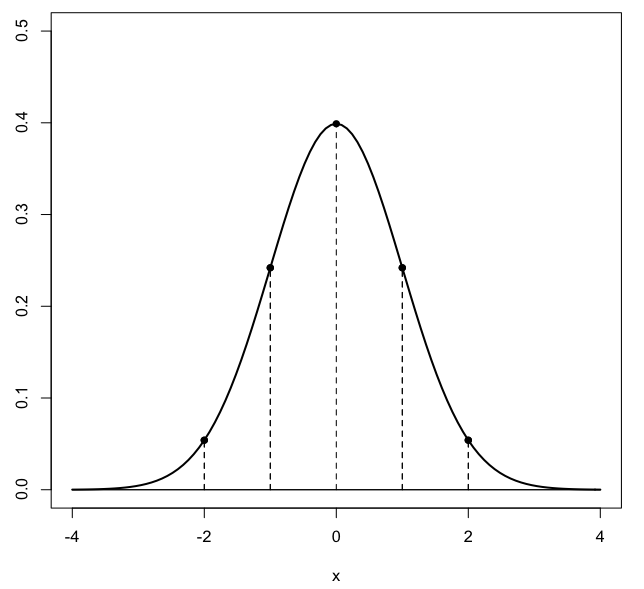
\includegraphics [scale=0.4] {gauss3.png} \end{center}

\title{Area of a circle}
\date{}

\begin{document}
\maketitle
\Large
In this first unit we will develop the most famous of Archimedes geometrical contributions, a theorem on the volume of the sphere.  

Before we get there, however, we need to spend some time with circles (also a topic to which he contributed) and look at the problem of the volume of cones and pyramids.  These are topics in geometry that come even before the volume of the sphere.

We start with the circle.  A fundamental result about circles is that the ratio of the circumference of a circle to its diameter is independent of the size of the circle.  
\begin{center}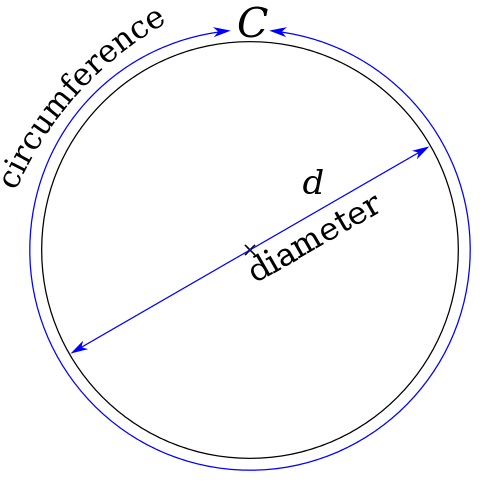
\includegraphics [scale=0.3] {circle0.png}\end{center}

The proportionality constant is 
\[ \pi d = C \]
Since the radius is one-half the diameter, $2r = d$ and
\[ 2 \pi r = C \]

This is usually stated as a self-evident fact, but it is actually a theorem to be proved.  We will need some of the apparatus of calculus to do that, so we defer the proof.

\subsection*{area of a circle}

Imagine dividing a circle into wedges, like you might do with a pizza.  Here, the pie has been divided into 16 parts.
\begin{center}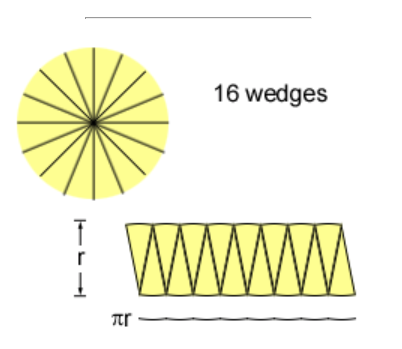
\includegraphics [scale=0.5] {circle_wedges.png}\end{center}

Since the pieces are triangular, it is easy to stack them next to each other with the bases and tips alternating, as shown.  Of course the bases are not straight, but have the same curvature as the edge of the circle.  

The length of the short side is the radius, $r$, and the length of the long side is approximately one-half the circumference so
\[ A =  r\cdot \frac{1}{2} \cdot 2 \pi r = \pi r^2 \]

The trick is to imagine that we subdivide the circle into many slices.  If there are infinitely many  slices, the edges will be  straight and this calculation becomes exact.

According to wikipedia

\url{https://en.wikipedia.org/wiki/Area_of_a_circle}

Eudoxus of Cnidus, born in the 5th century (408 BCE), proved that the area of a circle, like that of regular polygons, is proportional to both horizontal and vertical dimensions, and thus is proportional to the radius squared.

Somewhat later, it became clear that for a regular polygon, the area is equal to one-half the perimeter times the altitude from the center to each side (called the apothem).  Allowing the polygon to achieve many, many sides, that formula gives $1/2 \cdot 2 \pi r \cdot r = \pi r^2$.

The proof we gave above is very much like one attributed to Leonardo da Vinci, among others.

Another idea is to remove concentric strips from the edge and stack them.
\begin{center}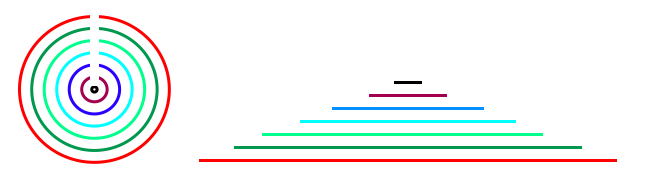
\includegraphics [scale=0.5] {circle_strips.png}\end{center}
We obtain a triangle of height $r$ and base $2 \pi r$ so its area is
\[ \frac{1}{2} \ 2 \pi r \cdot r = \pi r^2 \]

A proof that this triangle has the same area as the circle was given by Archimedes and is found in his \emph{Measurement of a Circle}, proposition 1.  However, many sources, including

\url{http://www.math.tamu.edu/~dallen/masters/Greek/eudoxus.pdf}

attribute the proof to Eudoxus, who was perhaps the second most famous mathematician of antiquity, and a colleague of Plato in Athens.

We'll look at the proof here even though it's a bit sophisticated for so early in the book, but the quote from Plutarch that follows is priceless.  It may be skipped (or skimmed) if you get bogged down.

$\circ$ \ Let $A$ be the area of the circle

$\circ$ \ Let $T$ be the area of the triangle formed with base $2 \pi r$ and height $r$ (i.e. the area of $T$ is $\pi r^2$).  

The method of proof is by finding a contradiction.  We will assume something next, and then prove that a contradiction results, so the assumption must be incorrect

$\circ$ \ Assume $A > T$.

That is, the difference $A - T$ is non-zero and positive: 
\[ A - T > 0 \]
Using the methods described \hyperref[sec:Archimedes_and_pi]{\textbf{here}}, we know that it is possible to construct an inscribed polygon whose area differs from $A$ by \emph{as little as we please}

\begin{center} 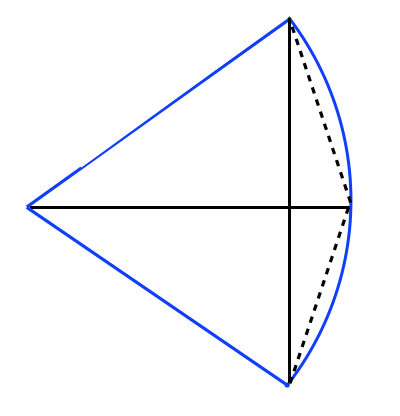
\includegraphics [scale=0.4] {inscribed_poly.png} \end{center}

In the figure, suppose that the black vertical is one side of an inscribed polygon of $n$ sides, and in the next step, we find a way to double the number of sides (dotted lines), thus, $6, 12, 24, 48, 96 \dots$ sides.

Clearly, the polygon with $2n$ sides is still contained within the circle, but its area more closely approximates that of the circle.  This can be repeated forever.

Call the area of the inscribed polygon $P$.  

So what we meant by as little as we please is that $P$ can be made closer to $A$ than $T$ is, simply on the assumption that $T < A$.  Since this is an \emph{inscribed} polygon, we have
\[ A - P < A - T \]
We must have that
\[ -P < -T \]
\[ T < P \]
(To see this last step, add $P + T$ to both sides).

However, for an inscribed polygon the perimeter is certainly less than the circumference of the circle and its apothem (the vertical to the sides of the polygon) is less than the radius of the circle.
\begin{center}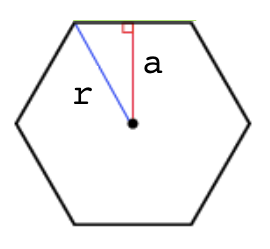
\includegraphics [scale=0.5] {apothem2.png}\end{center}
In the figure, it must be that $a < r$.  So

\[ P < \frac{1}{2} \cdot 2 \pi r \cdot r \]

By this second argument, we have shown that the area of the regular polygon, $P < T$.  However, we first showed that $T < P$.  We have reached a contradiction.  

Therefore, our assumption that $A > T$, is incorrect.
\[ A \ngtr T \]

A similar argument assuming $A < T$ also leads to a contradiction.  

Since $A$ is neither greater than nor smaller than $T$ it must be equal to $T$.
\[ A = T = \frac{1}{2} \cdot 2 \pi r \cdot r  = \pi r^2 \]

The analysis is taken from Dunham's \emph{Journey Through Genius}.  Here is a quote he presents from Plutarch, talking about Archimedes:

\begin{quote}It is not possible to find in all geometry more difficult and intricate questions, or more simple and lucid explanations. Some ascribe this to his natural genius; while others think that incredible effort and toil produced these, to all appearances, easy and unlabored results. No amount of investigation of yours would succeed in attaining the proof, and yet, once seen, you immediately believe you would have discovered it; by so smooth and so rapid a path he leads you to the conclusion required.\end{quote}

\end{document}